\documentclass[twoside]{book}

% Packages required by doxygen
\usepackage{fixltx2e}
\usepackage{calc}
\usepackage{doxygen}
\usepackage[export]{adjustbox} % also loads graphicx
\usepackage{graphicx}
\usepackage[utf8]{inputenc}
\usepackage{makeidx}
\usepackage{multicol}
\usepackage{multirow}
\PassOptionsToPackage{warn}{textcomp}
\usepackage{textcomp}
\usepackage[nointegrals]{wasysym}
\usepackage[table]{xcolor}

% Font selection
\usepackage[T1]{fontenc}
\usepackage[scaled=.90]{helvet}
\usepackage{courier}
\usepackage{amssymb}
\usepackage{sectsty}
\renewcommand{\familydefault}{\sfdefault}
\allsectionsfont{%
  \fontseries{bc}\selectfont%
  \color{darkgray}%
}
\renewcommand{\DoxyLabelFont}{%
  \fontseries{bc}\selectfont%
  \color{darkgray}%
}
\newcommand{\+}{\discretionary{\mbox{\scriptsize$\hookleftarrow$}}{}{}}

% Page & text layout
\usepackage{geometry}
\geometry{%
  a4paper,%
  top=2.5cm,%
  bottom=2.5cm,%
  left=2.5cm,%
  right=2.5cm%
}
\tolerance=750
\hfuzz=15pt
\hbadness=750
\setlength{\emergencystretch}{15pt}
\setlength{\parindent}{0cm}
\setlength{\parskip}{3ex plus 2ex minus 2ex}
\makeatletter
\renewcommand{\paragraph}{%
  \@startsection{paragraph}{4}{0ex}{-1.0ex}{1.0ex}{%
    \normalfont\normalsize\bfseries\SS@parafont%
  }%
}
\renewcommand{\subparagraph}{%
  \@startsection{subparagraph}{5}{0ex}{-1.0ex}{1.0ex}{%
    \normalfont\normalsize\bfseries\SS@subparafont%
  }%
}
\makeatother

% Headers & footers
\usepackage{fancyhdr}
\pagestyle{fancyplain}
\fancyhead[LE]{\fancyplain{}{\bfseries\thepage}}
\fancyhead[CE]{\fancyplain{}{}}
\fancyhead[RE]{\fancyplain{}{\bfseries\leftmark}}
\fancyhead[LO]{\fancyplain{}{\bfseries\rightmark}}
\fancyhead[CO]{\fancyplain{}{}}
\fancyhead[RO]{\fancyplain{}{\bfseries\thepage}}
\fancyfoot[LE]{\fancyplain{}{}}
\fancyfoot[CE]{\fancyplain{}{}}
\fancyfoot[RE]{\fancyplain{}{\bfseries\scriptsize Generated by Doxygen }}
\fancyfoot[LO]{\fancyplain{}{\bfseries\scriptsize Generated by Doxygen }}
\fancyfoot[CO]{\fancyplain{}{}}
\fancyfoot[RO]{\fancyplain{}{}}
\renewcommand{\footrulewidth}{0.4pt}
\renewcommand{\chaptermark}[1]{%
  \markboth{#1}{}%
}
\renewcommand{\sectionmark}[1]{%
  \markright{\thesection\ #1}%
}

% Indices & bibliography
\usepackage{natbib}
\usepackage[titles]{tocloft}
\setcounter{tocdepth}{3}
\setcounter{secnumdepth}{5}
\makeindex

% Custom commands
\newcommand{\clearemptydoublepage}{%
  \newpage{\pagestyle{empty}\cleardoublepage}%
}

\usepackage{caption}
\captionsetup{labelsep=space,justification=centering,font={bf},singlelinecheck=off,skip=4pt,position=top}

%===== C O N T E N T S =====

\begin{document}

% Titlepage & ToC
\pagenumbering{alph}
\begin{titlepage}
\vspace*{7cm}
\begin{center}%
{\Large Tratamento de classes abstratas }\\
\vspace*{1cm}
{\large Generated by Doxygen 1.8.14}\\
\end{center}
\end{titlepage}
\clearemptydoublepage
\pagenumbering{roman}
\tableofcontents
\clearemptydoublepage
\pagenumbering{arabic}

%--- Begin generated contents ---
\chapter{Hierarchical Index}
\section{Class Hierarchy}
This inheritance list is sorted roughly, but not completely, alphabetically\+:\begin{DoxyCompactList}
\item \contentsline{section}{Figura\+Geometrica}{\pageref{class_figura_geometrica}}{}
\begin{DoxyCompactList}
\item \contentsline{section}{Circulo}{\pageref{class_circulo}}{}
\item \contentsline{section}{Reta}{\pageref{class_reta}}{}
\item \contentsline{section}{Retangulo}{\pageref{class_retangulo}}{}
\end{DoxyCompactList}
\item \contentsline{section}{Screen}{\pageref{class_screen}}{}
\end{DoxyCompactList}

\chapter{Class Index}
\section{Class List}
Here are the classes, structs, unions and interfaces with brief descriptions\+:\begin{DoxyCompactList}
\item\contentsline{section}{\textbf{ Circulo} }{\pageref{class_circulo}}{}
\item\contentsline{section}{\textbf{ Figura\+Geometrica} }{\pageref{class_figura_geometrica}}{}
\item\contentsline{section}{\textbf{ Reta} }{\pageref{class_reta}}{}
\item\contentsline{section}{\textbf{ Retangulo} }{\pageref{class_retangulo}}{}
\item\contentsline{section}{\textbf{ Screen} }{\pageref{class_screen}}{}
\end{DoxyCompactList}

\chapter{File Index}
\section{File List}
Here is a list of all files with brief descriptions\+:\begin{DoxyCompactList}
\item\contentsline{section}{\textbf{ circulo.\+cpp} }{\pageref{circulo_8cpp}}{}
\item\contentsline{section}{\textbf{ circulo.\+h} }{\pageref{circulo_8h}}{}
\item\contentsline{section}{\textbf{ figurageometrica.\+cpp} }{\pageref{figurageometrica_8cpp}}{}
\item\contentsline{section}{\textbf{ figurageometrica.\+h} }{\pageref{figurageometrica_8h}}{}
\item\contentsline{section}{\textbf{ main.\+cpp} }{\pageref{main_8cpp}}{}
\item\contentsline{section}{\textbf{ reta.\+cpp} }{\pageref{reta_8cpp}}{}
\item\contentsline{section}{\textbf{ reta.\+h} }{\pageref{reta_8h}}{}
\item\contentsline{section}{\textbf{ retangulo.\+cpp} }{\pageref{retangulo_8cpp}}{}
\item\contentsline{section}{\textbf{ retangulo.\+h} }{\pageref{retangulo_8h}}{}
\item\contentsline{section}{\textbf{ screen.\+cpp} }{\pageref{screen_8cpp}}{}
\item\contentsline{section}{\textbf{ screen.\+h} }{\pageref{screen_8h}}{}
\end{DoxyCompactList}

\chapter{Class Documentation}
\section{Circulo Class Reference}
\label{class_circulo}\index{Circulo@{Circulo}}


{\ttfamily \#include $<$circulo.\+h$>$}

Inheritance diagram for Circulo\+:\begin{figure}[H]
\begin{center}
\leavevmode
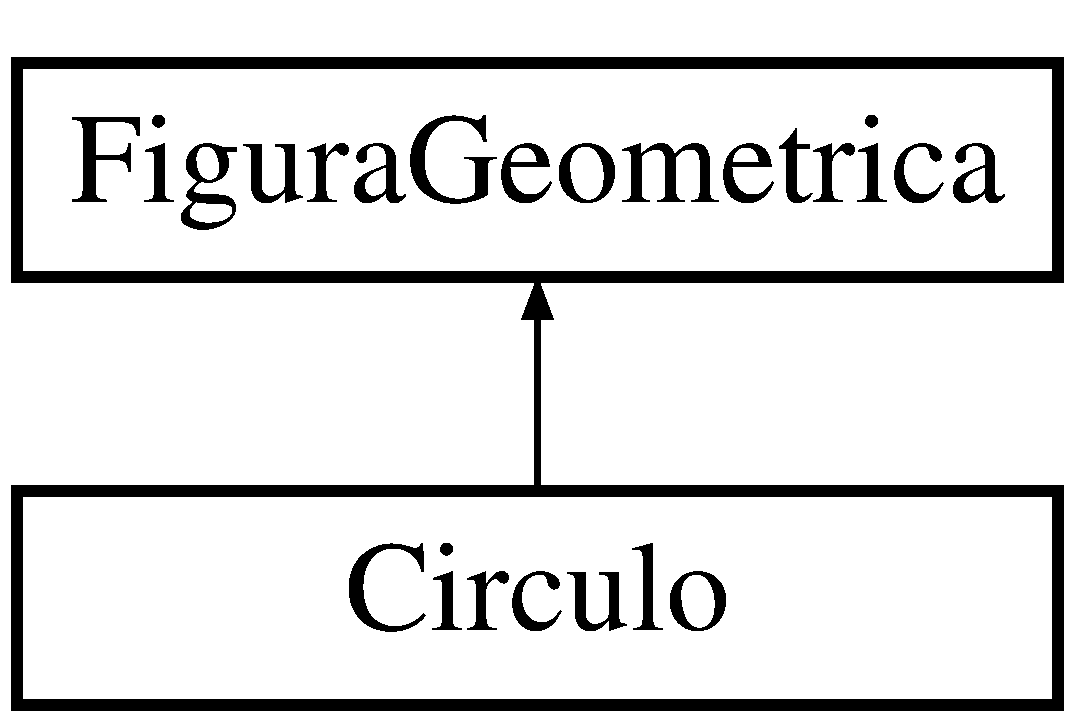
\includegraphics[height=2.000000cm]{class_circulo}
\end{center}
\end{figure}
\subsection*{Public Member Functions}
\begin{DoxyCompactItemize}
\item 
\textbf{ Circulo} (int x, int y, int r, int p)
\begin{DoxyCompactList}\small\item\em \doxyref{Circulo\+::\+Circulo}{p.}{class_circulo_a724022d12ca3c6a6ef37f132c837daf7} Construtor da classe circulo. \end{DoxyCompactList}\item 
void \textbf{ draw} (\textbf{ Screen} \&t)
\begin{DoxyCompactList}\small\item\em \doxyref{Circulo\+::draw}{p.}{class_circulo_a593787d6e0618c2eded23e8839e7bea6} -\/ Desenha o circulo na tela. \end{DoxyCompactList}\end{DoxyCompactItemize}


\subsection{Constructor \& Destructor Documentation}
\mbox{\label{class_circulo_a724022d12ca3c6a6ef37f132c837daf7}} 
\index{Circulo@{Circulo}!Circulo@{Circulo}}
\index{Circulo@{Circulo}!Circulo@{Circulo}}
\subsubsection{Circulo()}
{\footnotesize\ttfamily Circulo\+::\+Circulo (\begin{DoxyParamCaption}\item[{int}]{\+\_\+x,  }\item[{int}]{\+\_\+y,  }\item[{int}]{r,  }\item[{int}]{p }\end{DoxyParamCaption})}



\doxyref{Circulo\+::\+Circulo}{p.}{class_circulo_a724022d12ca3c6a6ef37f132c837daf7} Construtor da classe circulo. 


\begin{DoxyParams}{Parameters}
{\em \+\_\+x} & -\/ Coordenada x do centro \\
\hline
{\em \+\_\+y} & -\/ Coordenada y do centro \\
\hline
{\em r} & -\/ Raio do circulo \\
\hline
{\em p} & -\/\+Variavel responsavel por verificar se o circulo sera preenchido ou nao \\
\hline
\end{DoxyParams}


\subsection{Member Function Documentation}
\mbox{\label{class_circulo_a593787d6e0618c2eded23e8839e7bea6}} 
\index{Circulo@{Circulo}!draw@{draw}}
\index{draw@{draw}!Circulo@{Circulo}}
\subsubsection{draw()}
{\footnotesize\ttfamily void Circulo\+::draw (\begin{DoxyParamCaption}\item[{\textbf{ Screen} \&}]{t }\end{DoxyParamCaption})\hspace{0.3cm}{\ttfamily [virtual]}}



\doxyref{Circulo\+::draw}{p.}{class_circulo_a593787d6e0618c2eded23e8839e7bea6} -\/ Desenha o circulo na tela. 


\begin{DoxyParams}{Parameters}
{\em t} & -\/ Responsavel por inserir o circulo no painel(matriz) alocada na classe \doxyref{Screen}{p.}{class_screen} \\
\hline
\end{DoxyParams}


Implements \textbf{ Figura\+Geometrica} \doxyref{}{p.}{class_figura_geometrica_a8ee8dedc060b6059a805ea091aef2c41}.



The documentation for this class was generated from the following files\+:\begin{DoxyCompactItemize}
\item 
\textbf{ circulo.\+h}\item 
\textbf{ circulo.\+cpp}\end{DoxyCompactItemize}

\section{Figura\+Geometrica Class Reference}
\label{class_figura_geometrica}\index{Figura\+Geometrica@{Figura\+Geometrica}}


{\ttfamily \#include $<$figurageometrica.\+h$>$}

Inheritance diagram for Figura\+Geometrica\+:\begin{figure}[H]
\begin{center}
\leavevmode
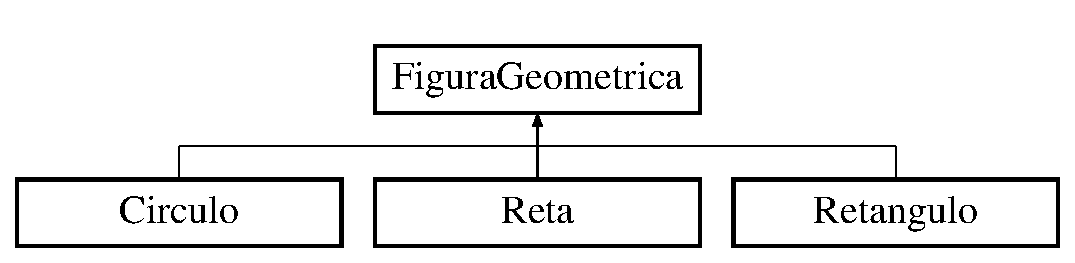
\includegraphics[height=2.000000cm]{class_figura_geometrica}
\end{center}
\end{figure}
\subsection*{Public Member Functions}
\begin{DoxyCompactItemize}
\item 
\textbf{ Figura\+Geometrica} ()
\item 
virtual void \textbf{ draw} (\textbf{ Screen} \&t)=0
\end{DoxyCompactItemize}


\subsection{Constructor \& Destructor Documentation}
\mbox{\label{class_figura_geometrica_a81d7c7efaea511e60a15f5a363138dd9}} 
\index{Figura\+Geometrica@{Figura\+Geometrica}!Figura\+Geometrica@{Figura\+Geometrica}}
\index{Figura\+Geometrica@{Figura\+Geometrica}!Figura\+Geometrica@{Figura\+Geometrica}}
\subsubsection{Figura\+Geometrica()}
{\footnotesize\ttfamily Figura\+Geometrica\+::\+Figura\+Geometrica (\begin{DoxyParamCaption}{ }\end{DoxyParamCaption})}



\subsection{Member Function Documentation}
\mbox{\label{class_figura_geometrica_a8ee8dedc060b6059a805ea091aef2c41}} 
\index{Figura\+Geometrica@{Figura\+Geometrica}!draw@{draw}}
\index{draw@{draw}!Figura\+Geometrica@{Figura\+Geometrica}}
\subsubsection{draw()}
{\footnotesize\ttfamily virtual void Figura\+Geometrica\+::draw (\begin{DoxyParamCaption}\item[{\textbf{ Screen} \&}]{t }\end{DoxyParamCaption})\hspace{0.3cm}{\ttfamily [pure virtual]}}



Implemented in \textbf{ Circulo} \doxyref{}{p.}{class_circulo_a593787d6e0618c2eded23e8839e7bea6}, \textbf{ Reta} \doxyref{}{p.}{class_reta_ac2e9805183cd474b62bffd8b032cd780}, and \textbf{ Retangulo} \doxyref{}{p.}{class_retangulo_ac088dd6d3f4f3d3f80363a868c2e74f1}.



The documentation for this class was generated from the following files\+:\begin{DoxyCompactItemize}
\item 
\textbf{ figurageometrica.\+h}\item 
\textbf{ figurageometrica.\+cpp}\end{DoxyCompactItemize}

\section{Reta Class Reference}
\label{class_reta}\index{Reta@{Reta}}


{\ttfamily \#include $<$reta.\+h$>$}

Inheritance diagram for Reta\+:\begin{figure}[H]
\begin{center}
\leavevmode
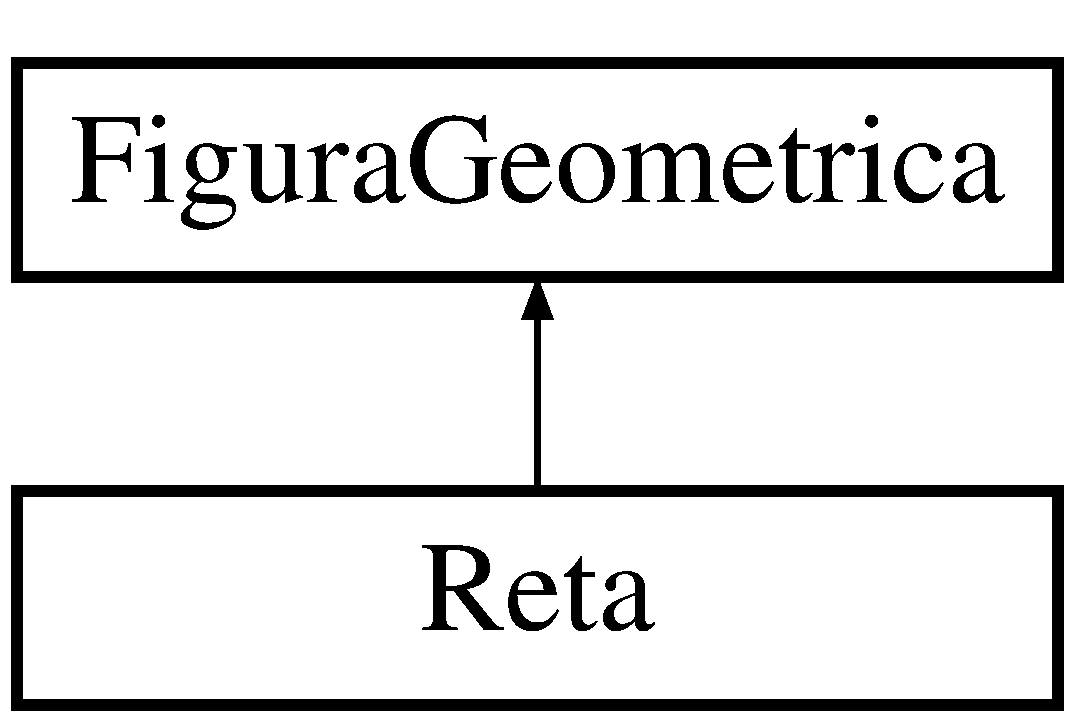
\includegraphics[height=2.000000cm]{class_reta}
\end{center}
\end{figure}
\subsection*{Public Member Functions}
\begin{DoxyCompactItemize}
\item 
\textbf{ Reta} (int x1, int y1, int x2, int y2)
\begin{DoxyCompactList}\small\item\em \doxyref{Reta\+::\+Reta}{p.}{class_reta_aa5d7a9cab70189356fc553bbb0a17fcd}. \end{DoxyCompactList}\item 
virtual void \textbf{ draw} (\textbf{ Screen} \&t)
\begin{DoxyCompactList}\small\item\em \doxyref{Reta\+::draw}{p.}{class_reta_ac2e9805183cd474b62bffd8b032cd780} -\/ Desenha a reta tendo como base o algoritmo de Bresenham. \end{DoxyCompactList}\end{DoxyCompactItemize}


\subsection{Constructor \& Destructor Documentation}
\mbox{\label{class_reta_aa5d7a9cab70189356fc553bbb0a17fcd}} 
\index{Reta@{Reta}!Reta@{Reta}}
\index{Reta@{Reta}!Reta@{Reta}}
\subsubsection{Reta()}
{\footnotesize\ttfamily Reta\+::\+Reta (\begin{DoxyParamCaption}\item[{int}]{\+\_\+x1,  }\item[{int}]{\+\_\+y1,  }\item[{int}]{\+\_\+x2,  }\item[{int}]{\+\_\+y2 }\end{DoxyParamCaption})}



\doxyref{Reta\+::\+Reta}{p.}{class_reta_aa5d7a9cab70189356fc553bbb0a17fcd}. 


\begin{DoxyParams}{Parameters}
{\em \+\_\+x1} & -\/ Coordenada X do ponto inicial \\
\hline
{\em \+\_\+y1} & -\/ Coordenada y do ponto inicial \\
\hline
{\em \+\_\+x2} & -\/ Coordenada X do ponto final \\
\hline
{\em \+\_\+y2} & -\/ Coordenada Y do ponto final \\
\hline
\end{DoxyParams}


\subsection{Member Function Documentation}
\mbox{\label{class_reta_ac2e9805183cd474b62bffd8b032cd780}} 
\index{Reta@{Reta}!draw@{draw}}
\index{draw@{draw}!Reta@{Reta}}
\subsubsection{draw()}
{\footnotesize\ttfamily void Reta\+::draw (\begin{DoxyParamCaption}\item[{\textbf{ Screen} \&}]{t }\end{DoxyParamCaption})\hspace{0.3cm}{\ttfamily [virtual]}}



\doxyref{Reta\+::draw}{p.}{class_reta_ac2e9805183cd474b62bffd8b032cd780} -\/ Desenha a reta tendo como base o algoritmo de Bresenham. 


\begin{DoxyParams}{Parameters}
{\em t} & -\/ Seta na tela(matriz) o desenho da reta \\
\hline
\end{DoxyParams}


Implements \textbf{ Figura\+Geometrica} \doxyref{}{p.}{class_figura_geometrica_a8ee8dedc060b6059a805ea091aef2c41}.



The documentation for this class was generated from the following files\+:\begin{DoxyCompactItemize}
\item 
\textbf{ reta.\+h}\item 
\textbf{ reta.\+cpp}\end{DoxyCompactItemize}

\section{Retangulo Class Reference}
\label{class_retangulo}\index{Retangulo@{Retangulo}}


{\ttfamily \#include $<$retangulo.\+h$>$}

Inheritance diagram for Retangulo\+:\begin{figure}[H]
\begin{center}
\leavevmode
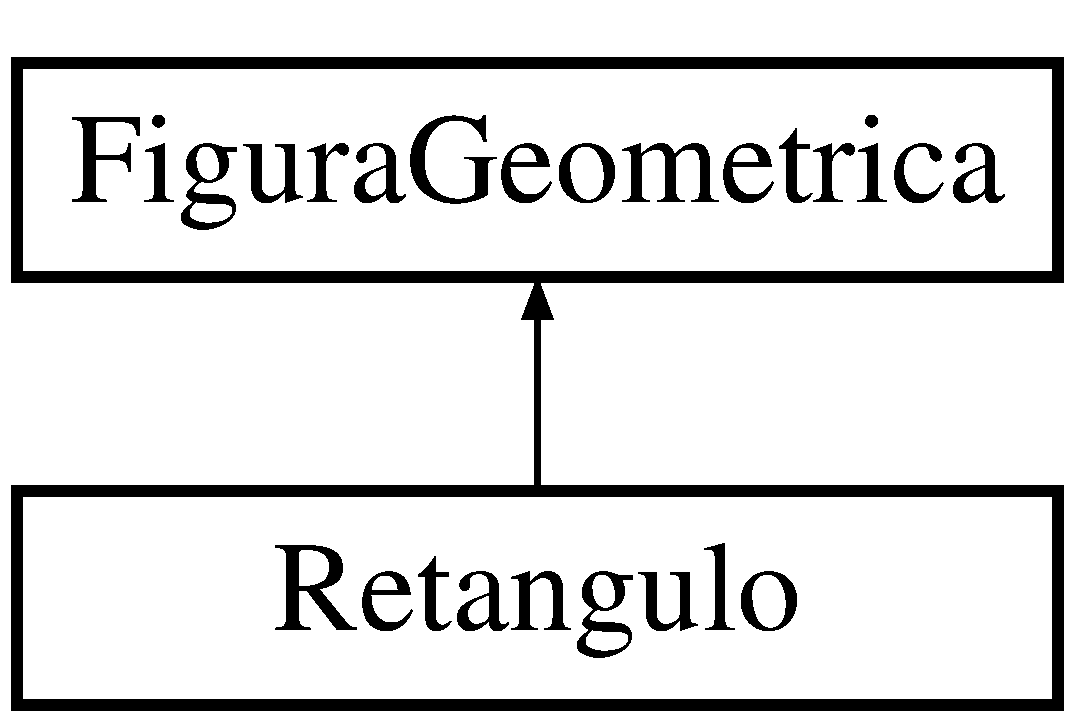
\includegraphics[height=2.000000cm]{class_retangulo}
\end{center}
\end{figure}
\subsection*{Public Member Functions}
\begin{DoxyCompactItemize}
\item 
\textbf{ Retangulo} (int x, int y, int larg, int alt, int aux)
\begin{DoxyCompactList}\small\item\em \doxyref{Retangulo\+::\+Retangulo}{p.}{class_retangulo_a5533c28fd6bf3dba362565351c2883dc} -\/ Construtor da classe retangulo. \end{DoxyCompactList}\item 
virtual void \textbf{ draw} (\textbf{ Screen} \&t)
\begin{DoxyCompactList}\small\item\em \doxyref{Retangulo\+::draw}{p.}{class_retangulo_ac088dd6d3f4f3d3f80363a868c2e74f1} -\/ Desenha o retangulo de acordo com o algoritmo implementado. \end{DoxyCompactList}\end{DoxyCompactItemize}


\subsection{Constructor \& Destructor Documentation}
\mbox{\label{class_retangulo_a5533c28fd6bf3dba362565351c2883dc}} 
\index{Retangulo@{Retangulo}!Retangulo@{Retangulo}}
\index{Retangulo@{Retangulo}!Retangulo@{Retangulo}}
\subsubsection{Retangulo()}
{\footnotesize\ttfamily Retangulo\+::\+Retangulo (\begin{DoxyParamCaption}\item[{int}]{\+\_\+x,  }\item[{int}]{\+\_\+y,  }\item[{int}]{\+\_\+larg,  }\item[{int}]{\+\_\+alt,  }\item[{int}]{\+\_\+aux }\end{DoxyParamCaption})}



\doxyref{Retangulo\+::\+Retangulo}{p.}{class_retangulo_a5533c28fd6bf3dba362565351c2883dc} -\/ Construtor da classe retangulo. 


\begin{DoxyParams}{Parameters}
{\em \+\_\+x} & -\/ Coordenada x onde o retangulo sera iniciado \\
\hline
{\em \+\_\+y} & -\/ Coordenada y onde o retangulo sera iniciado \\
\hline
{\em \+\_\+larg} & -\/ Largura do retangulo \\
\hline
{\em \+\_\+alt} & -\/ Altura do retangulo \\
\hline
{\em \+\_\+aux} & -\/ Variavel responsavel por verificar se o retangulo sera preenchido ou não \\
\hline
\end{DoxyParams}


\subsection{Member Function Documentation}
\mbox{\label{class_retangulo_ac088dd6d3f4f3d3f80363a868c2e74f1}} 
\index{Retangulo@{Retangulo}!draw@{draw}}
\index{draw@{draw}!Retangulo@{Retangulo}}
\subsubsection{draw()}
{\footnotesize\ttfamily void Retangulo\+::draw (\begin{DoxyParamCaption}\item[{\textbf{ Screen} \&}]{t }\end{DoxyParamCaption})\hspace{0.3cm}{\ttfamily [virtual]}}



\doxyref{Retangulo\+::draw}{p.}{class_retangulo_ac088dd6d3f4f3d3f80363a868c2e74f1} -\/ Desenha o retangulo de acordo com o algoritmo implementado. 


\begin{DoxyParams}{Parameters}
{\em t} & -\/ Desenha o retangulo na tela(matriz) \\
\hline
\end{DoxyParams}


Implements \textbf{ Figura\+Geometrica} \doxyref{}{p.}{class_figura_geometrica_a8ee8dedc060b6059a805ea091aef2c41}.



The documentation for this class was generated from the following files\+:\begin{DoxyCompactItemize}
\item 
\textbf{ retangulo.\+h}\item 
\textbf{ retangulo.\+cpp}\end{DoxyCompactItemize}

\section{Screen Class Reference}
\label{class_screen}\index{Screen@{Screen}}


{\ttfamily \#include $<$screen.\+h$>$}

\subsection*{Public Member Functions}
\begin{DoxyCompactItemize}
\item 
\textbf{ Screen} (int numlin, int numcol)
\begin{DoxyCompactList}\small\item\em \doxyref{Screen\+::\+Screen}{p.}{class_screen_a0d54b8e0c04b70a865538119464cf633} -\/ Contrutor da classe \doxyref{Screen}{p.}{class_screen}. \end{DoxyCompactList}\item 
void \textbf{ set\+Pixel} (int x, int y)
\begin{DoxyCompactList}\small\item\em \doxyref{Screen\+::set\+Pixel}{p.}{class_screen_ae6bea81c57a22d226507c3c26fa95ee0} -\/ Inseri um valor a cada elemento da matriz. \end{DoxyCompactList}\item 
void \textbf{ clear} ()
\begin{DoxyCompactList}\small\item\em \doxyref{Screen\+::clear}{p.}{class_screen_a35e74266b2a04e37b354ceff7a5f1031} -\/ Limpa toda a matriz colocando em cada elemento um espaço. \end{DoxyCompactList}\item 
void \textbf{ set\+Brush} (char brush)
\begin{DoxyCompactList}\small\item\em \doxyref{Screen\+::set\+Brush}{p.}{class_screen_a14a00e158f99df199772172554a20576} -\/ Seta um valor que vai ser inserido posteriormente a cada elemento da matriz. \end{DoxyCompactList}\end{DoxyCompactItemize}
\subsection*{Friends}
\begin{DoxyCompactItemize}
\item 
ostream \& \textbf{ operator$<$$<$} (ostream \&os, const \textbf{ Screen} \&t)
\end{DoxyCompactItemize}


\subsection{Constructor \& Destructor Documentation}
\mbox{\label{class_screen_a0d54b8e0c04b70a865538119464cf633}} 
\index{Screen@{Screen}!Screen@{Screen}}
\index{Screen@{Screen}!Screen@{Screen}}
\subsubsection{Screen()}
{\footnotesize\ttfamily Screen\+::\+Screen (\begin{DoxyParamCaption}\item[{int}]{\+\_\+numlin,  }\item[{int}]{\+\_\+numcol }\end{DoxyParamCaption})}



\doxyref{Screen\+::\+Screen}{p.}{class_screen_a0d54b8e0c04b70a865538119464cf633} -\/ Contrutor da classe \doxyref{Screen}{p.}{class_screen}. 


\begin{DoxyParams}{Parameters}
{\em numlin} & -\/ Numero de linhas da matriz \\
\hline
{\em numcol} & -\/ Numero de colunas \\
\hline
\end{DoxyParams}


\subsection{Member Function Documentation}
\mbox{\label{class_screen_a35e74266b2a04e37b354ceff7a5f1031}} 
\index{Screen@{Screen}!clear@{clear}}
\index{clear@{clear}!Screen@{Screen}}
\subsubsection{clear()}
{\footnotesize\ttfamily void Screen\+::clear (\begin{DoxyParamCaption}{ }\end{DoxyParamCaption})}



\doxyref{Screen\+::clear}{p.}{class_screen_a35e74266b2a04e37b354ceff7a5f1031} -\/ Limpa toda a matriz colocando em cada elemento um espaço. 

\mbox{\label{class_screen_a14a00e158f99df199772172554a20576}} 
\index{Screen@{Screen}!set\+Brush@{set\+Brush}}
\index{set\+Brush@{set\+Brush}!Screen@{Screen}}
\subsubsection{set\+Brush()}
{\footnotesize\ttfamily void Screen\+::set\+Brush (\begin{DoxyParamCaption}\item[{char}]{\+\_\+brush }\end{DoxyParamCaption})}



\doxyref{Screen\+::set\+Brush}{p.}{class_screen_a14a00e158f99df199772172554a20576} -\/ Seta um valor que vai ser inserido posteriormente a cada elemento da matriz. 


\begin{DoxyParams}{Parameters}
{\em \+\_\+brush} & -\/ Recebe o valor que ira ser setado \\
\hline
\end{DoxyParams}
\mbox{\label{class_screen_ae6bea81c57a22d226507c3c26fa95ee0}} 
\index{Screen@{Screen}!set\+Pixel@{set\+Pixel}}
\index{set\+Pixel@{set\+Pixel}!Screen@{Screen}}
\subsubsection{set\+Pixel()}
{\footnotesize\ttfamily void Screen\+::set\+Pixel (\begin{DoxyParamCaption}\item[{int}]{x,  }\item[{int}]{y }\end{DoxyParamCaption})}



\doxyref{Screen\+::set\+Pixel}{p.}{class_screen_ae6bea81c57a22d226507c3c26fa95ee0} -\/ Inseri um valor a cada elemento da matriz. 


\begin{DoxyParams}{Parameters}
{\em x} & -\/ Coordebada x do elemento \\
\hline
{\em y} & -\/ Coordenada y do elemento \\
\hline
\end{DoxyParams}


\subsection{Friends And Related Function Documentation}
\mbox{\label{class_screen_a97d31a27f2fd6c2032c87df591776aa6}} 
\index{Screen@{Screen}!operator$<$$<$@{operator$<$$<$}}
\index{operator$<$$<$@{operator$<$$<$}!Screen@{Screen}}
\subsubsection{operator$<$$<$}
{\footnotesize\ttfamily ostream\& operator$<$$<$ (\begin{DoxyParamCaption}\item[{ostream \&}]{os,  }\item[{const \textbf{ Screen} \&}]{t }\end{DoxyParamCaption})\hspace{0.3cm}{\ttfamily [friend]}}



The documentation for this class was generated from the following files\+:\begin{DoxyCompactItemize}
\item 
\textbf{ screen.\+h}\item 
\textbf{ screen.\+cpp}\end{DoxyCompactItemize}

\chapter{File Documentation}
\section{circulo.\+cpp File Reference}
\label{circulo_8cpp}\index{circulo.\+cpp@{circulo.\+cpp}}
{\ttfamily \#include \char`\"{}circulo.\+h\char`\"{}}\newline
{\ttfamily \#include $<$cmath$>$}\newline

\section{circulo.\+h File Reference}
\label{circulo_8h}\index{circulo.\+h@{circulo.\+h}}
{\ttfamily \#include $<$figurageometrica.\+h$>$}\newline
\subsection*{Classes}
\begin{DoxyCompactItemize}
\item 
class \textbf{ Circulo}
\end{DoxyCompactItemize}

\section{figurageometrica.\+cpp File Reference}
\label{figurageometrica_8cpp}\index{figurageometrica.\+cpp@{figurageometrica.\+cpp}}
{\ttfamily \#include \char`\"{}figurageometrica.\+h\char`\"{}}\newline

\section{figurageometrica.\+h File Reference}
\label{figurageometrica_8h}\index{figurageometrica.\+h@{figurageometrica.\+h}}
{\ttfamily \#include $<$screen.\+h$>$}\newline
\subsection*{Classes}
\begin{DoxyCompactItemize}
\item 
class \textbf{ Figura\+Geometrica}
\end{DoxyCompactItemize}

\section{main.\+cpp File Reference}
\label{main_8cpp}\index{main.\+cpp@{main.\+cpp}}
{\ttfamily \#include \char`\"{}mainwindow.\+h\char`\"{}}\newline
{\ttfamily \#include $<$Q\+Application$>$}\newline
\subsection*{Functions}
\begin{DoxyCompactItemize}
\item 
int \textbf{ main} (int argc, char $\ast$argv[$\,$])
\end{DoxyCompactItemize}


\subsection{Function Documentation}
\mbox{\label{main_8cpp_a0ddf1224851353fc92bfbff6f499fa97}} 
\index{main.\+cpp@{main.\+cpp}!main@{main}}
\index{main@{main}!main.\+cpp@{main.\+cpp}}
\subsubsection{main()}
{\footnotesize\ttfamily int main (\begin{DoxyParamCaption}\item[{int}]{argc,  }\item[{char $\ast$}]{argv[$\,$] }\end{DoxyParamCaption})}


\section{reta.\+cpp File Reference}
\label{reta_8cpp}\index{reta.\+cpp@{reta.\+cpp}}
{\ttfamily \#include \char`\"{}reta.\+h\char`\"{}}\newline
\subsection*{Macros}
\begin{DoxyCompactItemize}
\item 
\#define \textbf{ sgn}(x)~((x$<$0)?-\/1\+:((x$>$0)?1\+:0))
\end{DoxyCompactItemize}


\subsection{Macro Definition Documentation}
\mbox{\label{reta_8cpp_ae1b5a554c1d4d97654c06032a92f800a}} 
\index{reta.\+cpp@{reta.\+cpp}!sgn@{sgn}}
\index{sgn@{sgn}!reta.\+cpp@{reta.\+cpp}}
\subsubsection{sgn}
{\footnotesize\ttfamily \#define sgn(\begin{DoxyParamCaption}\item[{}]{x }\end{DoxyParamCaption})~((x$<$0)?-\/1\+:((x$>$0)?1\+:0))}


\section{reta.\+h File Reference}
\label{reta_8h}\index{reta.\+h@{reta.\+h}}
{\ttfamily \#include $<$figurageometrica.\+h$>$}\newline
\subsection*{Classes}
\begin{DoxyCompactItemize}
\item 
class \textbf{ Reta}
\end{DoxyCompactItemize}

\section{retangulo.\+cpp File Reference}
\label{retangulo_8cpp}\index{retangulo.\+cpp@{retangulo.\+cpp}}
{\ttfamily \#include \char`\"{}retangulo.\+h\char`\"{}}\newline
{\ttfamily \#include \char`\"{}reta.\+h\char`\"{}}\newline

\section{retangulo.\+h File Reference}
\label{retangulo_8h}\index{retangulo.\+h@{retangulo.\+h}}
{\ttfamily \#include $<$figurageometrica.\+h$>$}\newline
\subsection*{Classes}
\begin{DoxyCompactItemize}
\item 
class \textbf{ Retangulo}
\end{DoxyCompactItemize}

\section{screen.\+cpp File Reference}
\label{screen_8cpp}\index{screen.\+cpp@{screen.\+cpp}}
{\ttfamily \#include \char`\"{}screen.\+h\char`\"{}}\newline
{\ttfamily \#include $<$iostream$>$}\newline

\section{screen.\+h File Reference}
\label{screen_8h}\index{screen.\+h@{screen.\+h}}
{\ttfamily \#include $<$vector$>$}\newline
{\ttfamily \#include $<$iostream$>$}\newline
\subsection*{Classes}
\begin{DoxyCompactItemize}
\item 
class \textbf{ Screen}
\end{DoxyCompactItemize}

%--- End generated contents ---

% Index
\backmatter
\newpage
\phantomsection
\clearemptydoublepage
\addcontentsline{toc}{chapter}{Index}
\printindex

\end{document}
